\documentclass[12pt,a4paper]{report}
\usepackage[utf8]{inputenc}
\usepackage[T1]{fontenc}
\usepackage{xcolor}
\usepackage{graphicx}
\usepackage[french]{babel}
\usepackage{amsmath}
\usepackage{dirtree}
%\usepackage{esint}

\title{ \Huge \textbf{Rapport PlagueINT} \\ \large Modélisation de la propagation des épidémies}
%\date{\today}
\author{
CHERRE Romain
\and COROLLER Stevan 
\and PAMART Pierrick
\and PIPEREAU Yohan
\and \\
Encadrant: Mr. Vincent Gauthier }


\begin{document}
\maketitle

\tableofcontents

\newpage

\chapter*{Pré-Rapport}
\addcontentsline{toc}{chapter}{Pré-Rapport}

\section*{Analyse des besoins}

\subsection*{Fonction du produit}
\begin{flushleft}
  \begin{itemize}
	\item[$\bullet$] Mode de visualisation (écoulement du temps) 
	\item[$\bullet$] Modélisation mondiale avec cellules de la taille d'un pays
	\item[$\bullet$] Possibilité d'exporter le résultat dans un fichier lisible 
	\item[$\bullet$] Voies de transports prises en compte 
	\item[$\bullet$] Possibilité d'ajouter des événements (blocage d'aéroports, gare, etc..) au début de la modélisation
  \end{itemize}
\end{flushleft}

\subsection*{Contraintes techniques}
\begin{flushleft}
  \begin{itemize}
	\item[$\bullet$] Utiliser Java8 avec Eclipse et éventuellement d'autres languages si nécessaires 
	\item[$\bullet$] Possibilité d'exécution en mode terminal puis graphique
	\item[$\bullet$] Portabilité Windows, Linux, MAC OS (gérée nativement par Java)
    \end{itemize}
\end{flushleft}

\subsection*{Critères d'acceptabilité et de réception}
\begin{flushleft}
  \begin{itemize}
	\item[$\bullet$] Application performante avec un temps d'exécution raisonnable \\
	\item[$\bullet$] L'interface de l'application doit être conforme à la maquette suivante :\\
\subparagraph*{
------ Simulation de propagation de maladies ------\\
(1) Lancer la simulation\\
(2) Paramètres de simulation\\
(3) Quitter la simulation\\
}
\subparagraph*{  
------ Paramètres de simulation ------\\
(1) Quitter les options sans sauvegarder\\
(2) Date de début et durée de la simulation\\
(3) Pays infectés et nombre d'infectés de départ\\
(4) Choisir les constantes de propagation\\
(5) Gérer les évènements\\
(6) Choisir une maladie pré-enregistrée\\
(7) Quitter et sauvegarder les paramètres\\
}
\subparagraph*{  
------ Evènements ------\\
(1) Créer un évènement\\
(2) Voir les évènements\\
(3) Supprimer un évènement\\
(4) Revenir aux paramètres\\
}
\subparagraph*{  
------ Résultat de la simulation ------\\
(1) Voir la carte du monde\\
(2) Voir les statistiques globales\\
(3) Voir les statistiques d'un pays\\
(4) Extraire le résultat dans un fichier .csv\\
(5) Revenir au menu principal\\
}
  \end{itemize}
\end{flushleft}

\subsection*{Extensions}
\begin{flushleft}
  \begin{itemize}
	\item[$\bullet$] Interface - graphique 
	\item[$\bullet$] Informations sur les celulles (petits graphiques, etc...) 
	\item[$\bullet$] Modification de l'environnement (hygiène, température, etc...) 
  \end{itemize}
\end{flushleft}

\subsection*{Juridique}
\begin{flushleft}
Creative Commons sans usage commercial [BY NC SA]
\end{flushleft}

\section*{Spécification fonctionnelle générale}

\subsection*{Fonction du produit}
	\begin{flushleft}
	Pour l'écoulement du temps, nous avons choisi de discrétiser le temps. \\
	Pour l'importation des données et leur traitement, Python est fortement envisagé en tant qu'outil plus performant que Java à l'aide de certaines bibliothèques précodées.
	Pour l'exportation des résultats dans un fichier lisible, on exporterait les données dans un fichier csv en utilisant des fonctionnalités de lecture/écriture de fichier.\\
	Pour modéliser les voies de transports, on utiliserait un seul graphe avec comme noeuds du graphe les pays et sur les branches, le nombre de passagers par jour.
	\end{flushleft}

\subsection*{Critères d'acceptabilité et de réception}
\begin{flushleft}
	Pour la résolution des équations différentielles, on utiliserait dans un premier temps une méthode d'Euler. Dans un second temps, on implémenterait une méthode de Runge Kutta qui nous permettrait de gagner en précision. \\
	Pour l'interface utilisateur, on permettrait à l'utilisateur de définir l'échelle de temps afin de gérer la rapidité du programme. L'utilisateur pourrait également choisir les pays de lancement de la maladie. Il écrirait le nom du pays et on vérifierait si le nom correspond au nom d'un pays présent dans la liste d'une variable pays. \\
	Enfin pour les coefficients de propagation des différentes maladies, il y a le mode manuel ou l'utilisateur saisit les coefficients à la main et lance ensuite notre programme de modélisation. Mais il y a aussi le mode d'utilisation où l'utilisateur 
rentre la maladie et où le programme va chercher dans des données que l'on a générées précédemment à partir de statistiques mondiales sur les maladies.
\end{flushleft}

\subsection*{Extensions}
\begin{flushleft}
 	Pour l'interface graphique qui permettra d'afficher une carte du monde ainsi que de tracer des graphiques relatifs aux données de la celulle et leur évolution dans le temps, nous utiliserons la librairie (toolkit) graphique JavaFX. \\
	Pour la modification de l'environnement (hygiène, température, etc...), on modifie directement les coefficients de propagation de la maladie dans la cellule.
\end{flushleft}

\section*{Regroupement modulaire des fonctionnalités}
\begin{flushleft}
	\begin{itemize}
		\item[$\bullet$] Visualisation
			\begin{itemize}
				\item Terminal
				\item Graphique
				\item Exportation en CSV
			\end{itemize}
		\item[$\bullet$] Évènements
			\begin{itemize}
				\item Blocage de lieux de transports
				\item Blocage des frontières
			\end{itemize}
		\item[$\bullet$] Statistiques
			\begin{itemize}
				\item Par pays : évolutions du nombre d'infectés, ...
				\item Générales
			\end{itemize}
		\item[$\bullet$] Calcul des évolutions temporelles
	\end{itemize}
\end{flushleft}

\section*{Description du flux des données entre les modules}

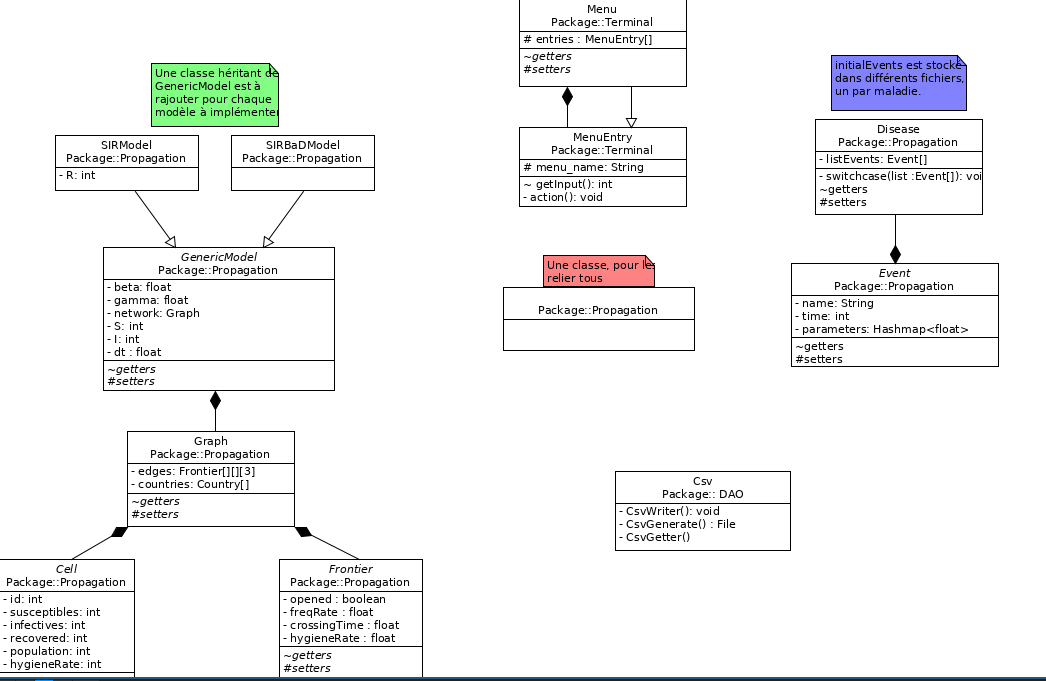
\includegraphics[angle=270 , scale=0.5]{uml.png}

\begin{flushleft}
	Le diagramme UML ci-dessus ne présente pas les relations entre toutes les classes car nous comptons voir comment regrouper certaines classes dans des phases ultérieures de notre développement.
\end{flushleft}


\chapter*{Conception détaillée}
\addcontentsline{toc}{chapter}{Conception détaillé}
\paragraph{Guide pour le développeur}

\begin{flushleft}
\begin{itemize}
L'aborescence des paquets est la suivante:
\item DAO: Data Access Object: Paquet contenant les classes relatives aux données. Dans notre projet les données sont stockées dans fichier .txt avec séparateurs.
\item Main: Contient la classe Context.java qui est itérée tous les dt et qui lance la création des objets et permet le déroulement du programme.
\item propagation: Ce paquet contient les éléments relatifs aux pays, frontières, les modèles épidémiques et les événements. Nous voulions modéliser trois types de frontières: Air, Land et Maritime. Les appels pour les extractions de données du CSV se font 
dans la classe Graph.java.
\item service: Ce paquet contient une première version de résolution des équations différentielles avant l'implémentation de utils.
\item terminal: Ce paquet contient l'ensemble des fonctions donnant le terminal utilisateur.
\item utils: Ce paquet contient les outils de résolution des équations différentielles en proposant une implémentation de la méthode d'Euler.
\end{itemize}
\end{flushleft}

\chapter*{Bilan}
\addcontentsline{toc}{chapter}{Bilan}

\paragraph{Comparaison entre l'objectif et la réalisation}
\begin{flushleft}
	Les contraintes techniques ont bien été respectées: utilisation de Java8 et Eclipse, possibilité d'exécution dans un terminal cependant la portatibilité Windows n'est pas garantie car l'arborescence utilise \ au lieu de /. Le programme fonctionne correctement sous Linux et MacOS. Nous n'avons pas eu le temps de travailler sur l'interface graphique, considéré comme une 
extension du programme. Il possible d'obtenir des graphes sur l'état des pays en récupérant les fichiers .csv de données et en utilisant un tableur. \newline
Concernant les critères d'acceptabilité et de réception, l'interface utilisateur ne correspond pas complètement à la maquette initiale: il ressemble à la maquette mais l'ordre des menus n'est pas le même, la version finale nous paraîssait plus logique et 
intuitive. La méthode d'Euler est implémentée, mais la méthode de Runge-Kutta, plus précise, ne l'est pas encore. \newline
Contrairement à ce qui était prévu, nous n'avons pas utilisé python pour importer et traiter les données dont nous nous servons. En effet, nous sommes tous habitués à utiliser bash en tant qu'outil natif en administraiton système. \newline
Enfin, à l'exception des différents modèles de propagation des maladies (notamment le modèle SIR avec naissances et morts), tous les choix possibles qui étaient prévus pour la modification des paramètres de propagation, et qui n'étaient pas considérés comme 
des extensions (comme le taux d'hygiène des pays et frontières) sont implémentés. \newline
La fonction d'importation des données est fonctionnelle. En particulier, nous avons essayé de trouver et parser des données réelles sans succès. Nous avons alors décidé de créer un monde fictif linuxmap. Ci-dessous la carte linuxmap:
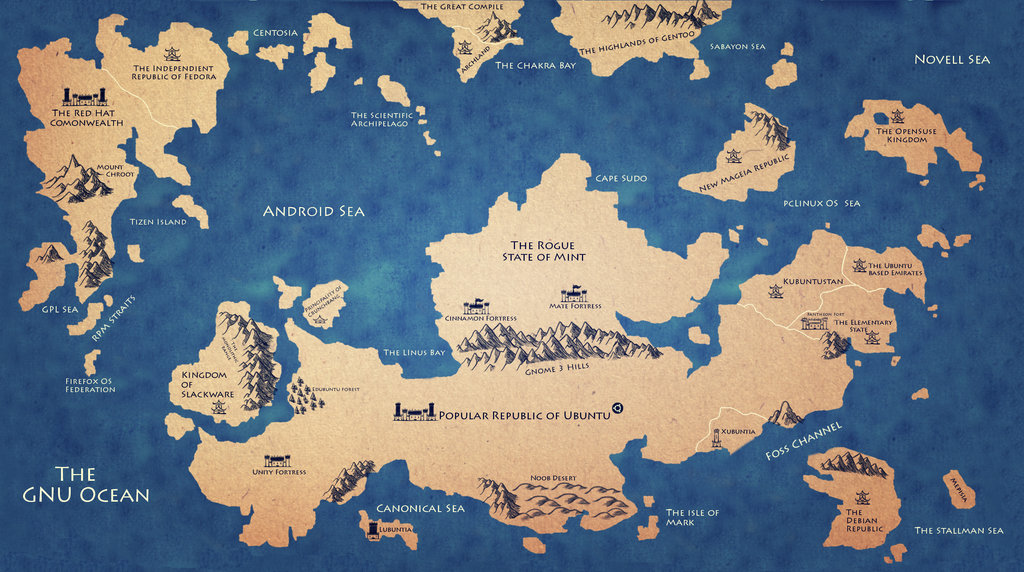
\includegraphics[angle=270 , scale=0.5]{linuxmap.jpg}


\end{flushleft}

\chapter*{Manuel utilisateur}
\addcontentsline{toc}{chapter}{Manuel utilisateur}

\paragraph{Guide d'utilisation du programme PlagueINT}

\section*{Aborescence des Menus}
\begin{flushleft}

L'interaction entre l'utilisateur et le programme se fait par l'utilisation d'un terminal divisés en menus.
\dirtree{%
.1 Gérer les événements .
.2 Lister et supprimer l'évenement choisi .
.3 Créer un événement .
.4 Moment de déclenchement .
.5 Constantes .
.6 Beta: coefficient de propagation .
.6 Gamma: coefficient de guérison .
.6 Mu: taux de mortalité .
.5 Paramètres du graphe .
.6 Pays1 .
.7 Population du pays .
.8 Nombre de sains .
.8 Nombre d'infectés .
.8 Nombre de guéris .
.7 Etat des frontières du pays .
.8 Frontière avec Pays1 .
.8 Frontière avec Pays2 .
.6 Pays2 .
.7 Population du pays .
.8 Nombre de sains .
.8 Nombre d'infectés .
.8 Nombre de guéris .
.7 Etat des frontières du pays .
.8 Frontière avec Pays1 .
.8 Frontière avec Pays2 .
.1 Personnalisation de la maladie .
.2 Paramètres de propagation .
.3 Choix d'un modèle .
.4 Modèle SIR  .
.4 Modèle SIR avec naissances et morts .
.3 Constantes .
.4 Beta: coefficient de propagation .
.4 Gamma: coefficient de guérison .
.4 Mu: taux de mortalité .
.3 Échelle de temps dt .
.2 Paramètres de départ .
.1 Choix de la maladie .
.2 Peste .
.2 Lèpre .
.1 Exporter les paramètres et évènements .
.1 Importer les paramètres et évènements .
.1 Lancer la simulation . 
}
\end{flushleft}

\begin{flushleft}
Le choix d'une maladie permet de charger les données pré-enregistrées (constantes, population de départ, évènements...) d'une maladie connue. Nous n'avons pas eu le temps de générer ces données, mais la fonctionnalité elle-même est implémentée. \newline
La personnalisation de la maladie permet de modifier les données de départ de la modélisation (que l'on ait choisi une maladie précédemment ou non). Ainsi on peut modifier l'état de départ des frontières (ouverture/fermeture et flux de population), la 
population de départ de tous les pays (répartie entre les sains, les infectés et les guéris) et les paramètres de propagation de la maladie (coefficients Beta et Gamma, Mu n'étant pas implémenté). \newline
Les événements sont des phénomènes modifiant les données du problème à un instant t. Ils permettent de modifier les mêmes paramètres que le menu de personnalisation de la maladie, mais à un instant donné non nul. \newline
Exporter les paramètres et évènements permet de sauvegarder les modifications apportées aux paramètres de la simulation, et importer les paramètres et évènements permet de charger les sauvegardes précédentes. \newline
	Lorsque l'utilisateur choisit simulation, il peut renseigner le nombre d'itérations qu'il veut faire. Les résultats sont exportés dans des fichiers CSV (un par pays) avec le temps et la répartition de population dans le dossier result.
\end{flushleft}

\begin{flushleft}
	Les test unitaires peuvent être exécutés dans DAO.CsvTest.
\end{flushleft}

\end{document}
